\documentclass[article,12pt]{elsarticle}
\usepackage[utf8]{inputenc}
\usepackage{graphicx}
\usepackage{booktabs}
\usepackage{subcaption}
\usepackage{amssymb}
\usepackage{flushend}
\usepackage{float}
\usepackage{amsmath}
\usepackage{amsfonts}
\usepackage{dcolumn}
\usepackage{amsthm}
\usepackage{caption}
\usepackage{lmodern}
\usepackage{booktabs}
\usepackage{color}
\usepackage{longtable}
\usepackage{rotating}
\usepackage{etoolbox}
\usepackage{hyperref}
\usepackage{comment}
\usepackage{pdflscape}
\usepackage{comment}
\usepackage[table,xcdraw]{xcolor}
\usepackage[framemethod=TikZ]{mdframed}
\usepackage[a4paper, left=1.5cm, right=1.5cm, top=2cm, bottom=2cm]{geometry}

\begin{document}

\mdfsetup{innertopmargin=10pt,linecolor=blue!20,%
linewidth=2pt,topline=true,
frametitleaboveskip=\dimexpr-\ht\strutbox\relax,}

\begin{frontmatter}
    \title{Laboratorio de Óptica \\  Práctica  IV: Índice de Refracción}
    \author{López González Andrés$^1$, Reyes Saldivar Ailton Uriel$^2$ y Gante Morales Pedro José$^3$} %Aquí va el nombre de los integrantes que participaron en el informe.
    \address{$^1$ Facultad de Ciencias, Universidad Nacional Autónoma de México, M\'exico CDMX.}

\begin{abstract}
En esta práctica de laboratorio se determinaron los índices de refracción de diferentes materiales utilizando cinco métodos experimentales. Los resultados obtenidos fueron: Reflexión Total Interna ($n = 1.4665 \pm 0.3925$), Método de Pfund ($n = 1.4816 \pm 0.029$), Profundidad Aparente ($n = 1.487 \pm 0.001$), Placa Plano Paralela ($n = 1.31 \pm 0.014$) y Método del Prisma ($n = 1.782 \pm 0.045$). Se observó que el método de Profundidad Aparente presentó la menor incertidumbre, mientras que Reflexión Total Interna tuvo la mayor imprecisión. Los valores obtenidos fueron consistentes con los teóricos dentro del margen de error experimental, lo que valida la efectividad de los métodos empleados.

\end{abstract}
    
\end{frontmatter}

\vspace{0.5cm} 



\section{Introducción}
El índice de refracción ($n$) es una propiedad óptica fundamental que describe cómo la luz cambia de velocidad al pasar de un medio a otro \cite{indice_ref}. Se define como:

\begin{mdframed}
\begin{equation}
    n = \frac{c}{v}
\end{equation}
\end{mdframed}

donde:
\begin{itemize}
    \item $c$ es la velocidad de la luz en el vacío ($3.00 \times 10^8$ m/s) \cite{snell}.
    \item $v$ es la velocidad de la luz en el medio.
\end{itemize}

Cuando un rayo de luz incide en la frontera entre dos medios, se refracta según la Ley de Snell \cite{snell}:

\begin{mdframed}
\begin{equation}
    n_I \sin\theta_I = n_T \sin\theta_T
\end{equation}
\end{mdframed}

Este fenómeno es la base para varios métodos de medición del índice de refracción \cite{indice_ref}. Estos métodos permiten caracterizar materiales translúcidos y tienen aplicaciones en diversos fenómenos ópticos, como espejismos, arcoíris y lentes \cite{indice_ref}.

\subsection*{Métodos de Medición del Índice de Refracción} \cite{indice_ref}
Se describen cinco métodos experimentales:

\subsection{Reflexión Total Interna} \cite{indice_ref}
Se utiliza un semicírculo de material translúcido y un láser. El ángulo crítico $\theta_c$ se determina cuando el rayo refractado se mueve paralelo a la interfaz. El índice de refracción del material se obtiene con:

\begin{mdframed}
\label{RTI}
\begin{equation}
    \theta_c = \arcsin\left(\frac{n_T}{n_I}\right)
\end{equation}
\end{mdframed}

donde $n_T$ es el índice del medio exterior (aire, $n \approx 1$).

\subsection{Método de Pfund} \cite{indice_ref}
Se utiliza una placa translúcida con una superficie rugosa en un lado. Un haz láser forma un halo circular debido a la reflexión total interna. El índice de refracción se obtiene con:

\begin{mdframed}
\label{Pfound}
\begin{equation}
    n_P = n_T \frac{\sqrt{D^2 + 16h^2}}{D}
\end{equation}

\end{mdframed}

donde $D$ es el diámetro del halo y $h$ el espesor de la placa.

\subsection{Método de Profundidad Aparente} \cite{indice_ref}
Se observa un objeto a través de una placa translúcida. Se mide la diferencia entre la profundidad real $r$ y la profundidad aparente $a$. El índice de refracción se calcula con:

\begin{mdframed}
\label{P.A}
\begin{equation}
    n_P = \frac{r}{a} n_T
\end{equation}
\end{mdframed}

\subsection{Método de la Placa Plano Paralela} \cite{indice_ref}
Se usa una placa rectangular en la que el haz de luz se desplaza lateralmente. La desviación depende de la geometría de la placa. La fórmula experimental para el índice de refracción es:

\begin{mdframed}
\label{PPP}
\begin{equation}
    n_P = n_I \left(\sin^2\theta_I + \left(\frac{D \sin\theta_I \cos\theta_I}{D \sin\theta_I - X} \right)^2\right)^{1/2}
\end{equation}
\end{mdframed}

donde $X$ es el desplazamiento lateral del haz.

\subsection{Método del Prisma} \cite{indice_ref}
Se hace pasar un haz de luz a través de un prisma óptico. Se mide el ángulo de desviación mínima $\delta_m$. El índice de refracción del prisma se obtiene con:

\begin{mdframed}
\label{Prisma}
\begin{equation}
    n = \frac{\sin\left(\frac{\delta_m + \alpha}{2} \right)}{\sin\left(\frac{\alpha}{2}\right)}
\end{equation}
\end{mdframed}

donde $\alpha$ es el ángulo del prisma.



\subsection{Hipótesis}

Dado que la luz cambia su dirección y velocidad al ingresar a un medio con un índice de refracción diferente, es posible determinar el índice de refracción de un material midiendo la desviación de un haz de luz mediante métodos experimentales.


\subsection{Objetivos}
\begin{itemize}
    \item Aplicar la Ley de Snell para calcular el índice de refracción en diferentes medios.
    \item Evaluar la precisión de distintos métodos experimentales de medición del índice de refracción.
    \item Comparar los resultados obtenidos con valores teóricos y bibliográficos.
\end{itemize}


\section{Desarrollo Experimental}
\subsection*{Método de Reflexión Total Interna}

Primero alineamos el haz Lasér con el eje cero del goniómetro, posteriormente colocamos la placa semicircular de acrílico sobre el goniómetro, de tal forma que la cara plana de la placa coincida con el eje de 90° del goniómetro y que la parte circular este del mismo lado donde se encuentra el Lasér. Luego se aumento gradualmente el ángulo de incidencia ($\theta_I$) hasta que el haz refractado desaparecio y solo se observara el haz reflejado figura 1. Este ángulo es el \textbf{ángulo crítico} ($\theta_c$).

\begin{figure}[H]
    \centering
    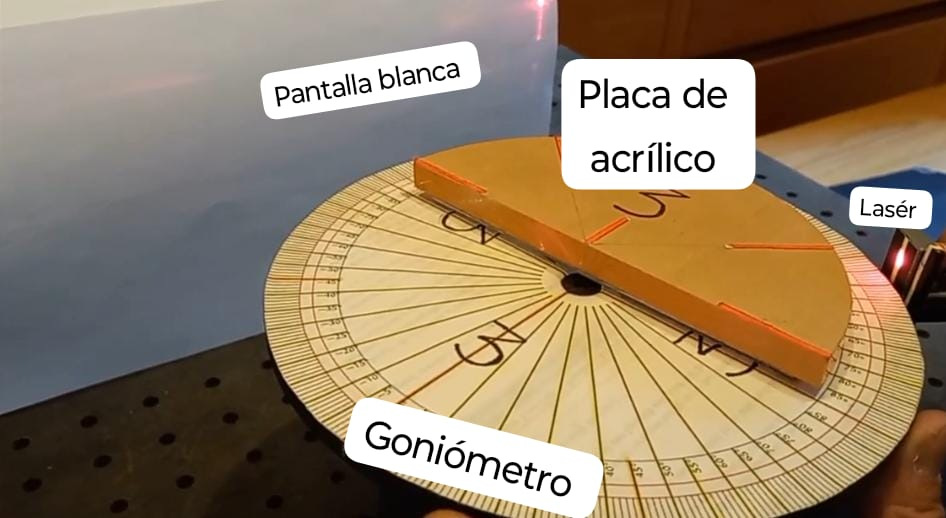
\includegraphics[width=0.5\linewidth]{RTI.png}
    \caption{
Montaje del areglo experimental cuando se tiene el ángulo crítico}
    \label{fig:enter-label}
\end{figure}

\subsection*{Método de Pfund}

Colocamos la placa de acrílico justo debajo del Laser, posteriormente colocamos papel higiénico sobre la placa y con ayuda de un gotero humedecimos el papel para asegurar que este hiciera contacto con la placa de esta manera se formo un halo sobre la superficie sperior de la placa (figura 2). Con ayuda de un vernier medimos el diamétro del halo. Por ultimo con ayuda del mismo vernier medimos el espesor de la placa de acrílico.

\begin{figure}[H]
    \centering
    
\includegraphics[width=0.5\linewidth]{image.png}
    \caption{Montaje experimental del método de pfund}
    \label{fig:enter-label}
\end{figure}

\subsection*{Placa Plano Paralela}

Primero alineamos el haz de Lasér con el eje cero del goniómetro luego colocamos una pantalla blanca del lado contrario al Lasér, posteriormente colocamos el recipiente con agua sobre el goniómetro de tal forma que una de sus caras coincidiera con el eje de noventa. Para la incidencia de 0° marcamos la posición del Lasér sobre la pantalla (posición inicial), luego fuimos aumentando el ángulo de incidencia de 5 en 5 (figura 3) grados hasta llegar a la marca de 40° y marcamos la posicion del haz sobre la pantalla para cada una de estas variaciones del ángulo incidente. Por ultimo medimos con la ayuda de un vernier la distancia para cada una de las marcas respecto a la posición inicial. 

\begin{figure}[H]
    \centering
    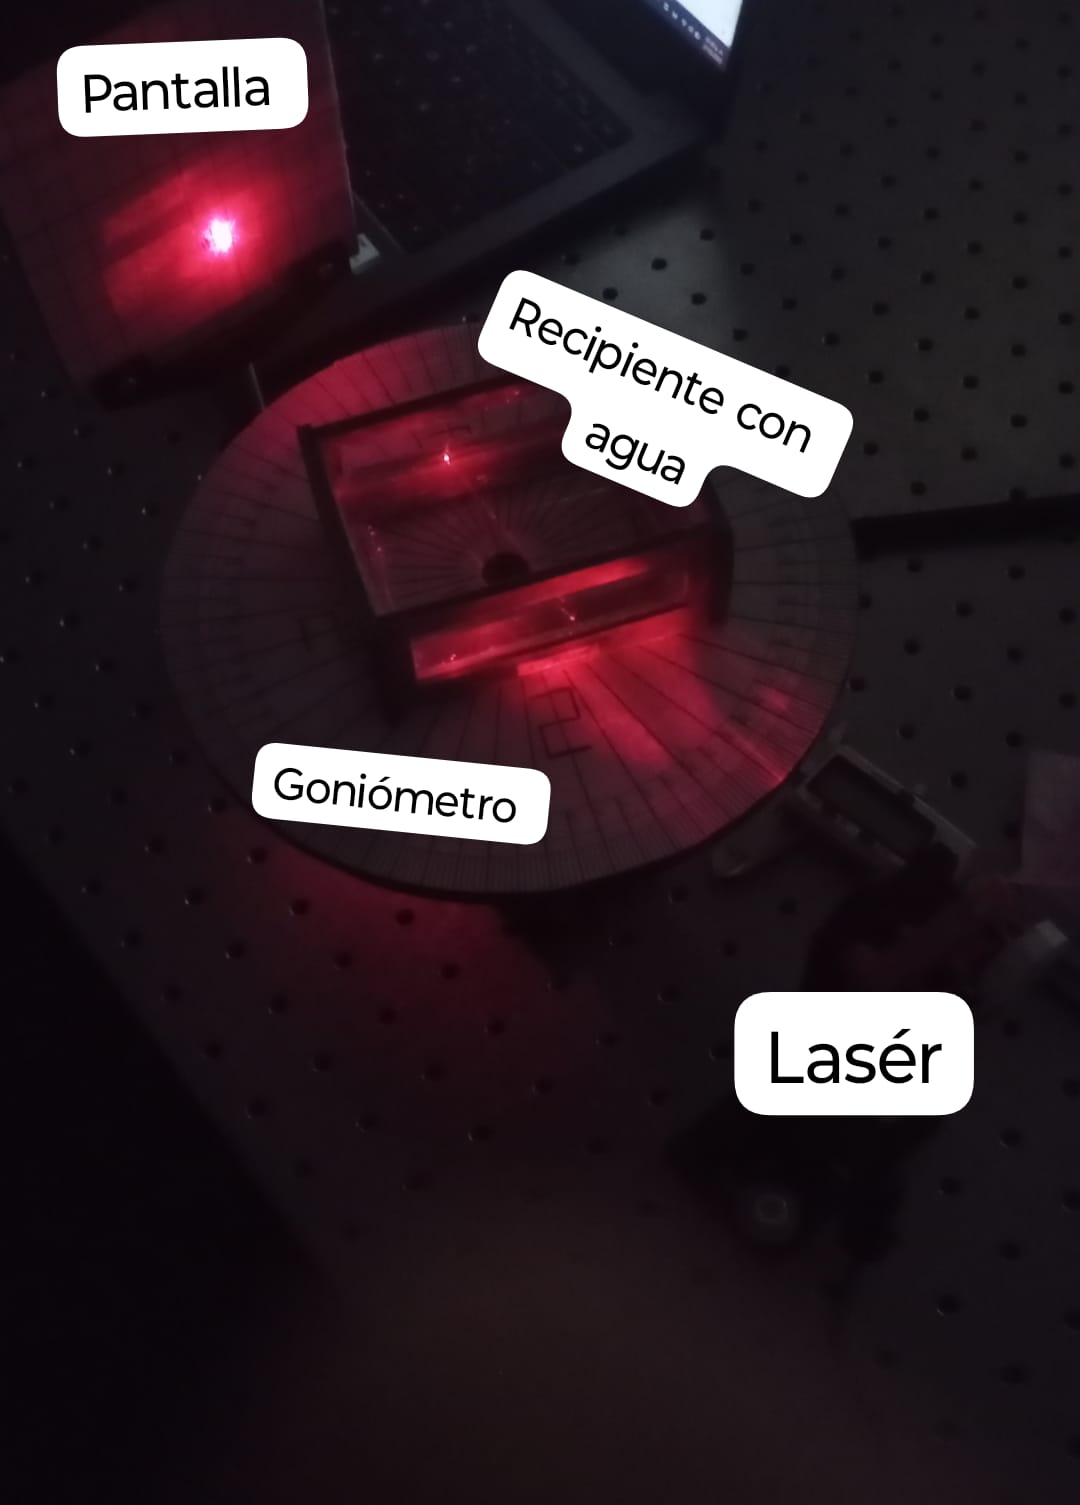
\includegraphics[width=0.3\linewidth]{PP.png}
    \caption{Areglo experimental para el método de placas plano paralelas}
    \label{fig:enter-label}
\end{figure}

\subsection*{Profundidad Aparente}

Primero colocamos una credencial bajo el microscopio y enfocamos las letras de la credencial moviendo el miscrospio ya sea manualmente o haciendo uso del tornillo de precision hasta que las letras se vieran lo más nítido posible, una vez enfocada la imagen medimos la posición de esta imagen usanso el vernier del miscroscopio está medida corresponde a la profundidad real respecto de la superficie superior de la placa de acrílico, luego colocamos la placa de acrílico sobre la credencial y repetimos el mismo proceso anterior obteniendo asi la profundiadad aparente de la imagen respecto a la superficie superior de la placa, por ulimo colocamos la credencial sobre la placa de acrílico y nuevamente enfocando las letras del la credencial se obtuvo la posición de la superficie superior de la placa. 

\begin{figure}[H]
    \centering
    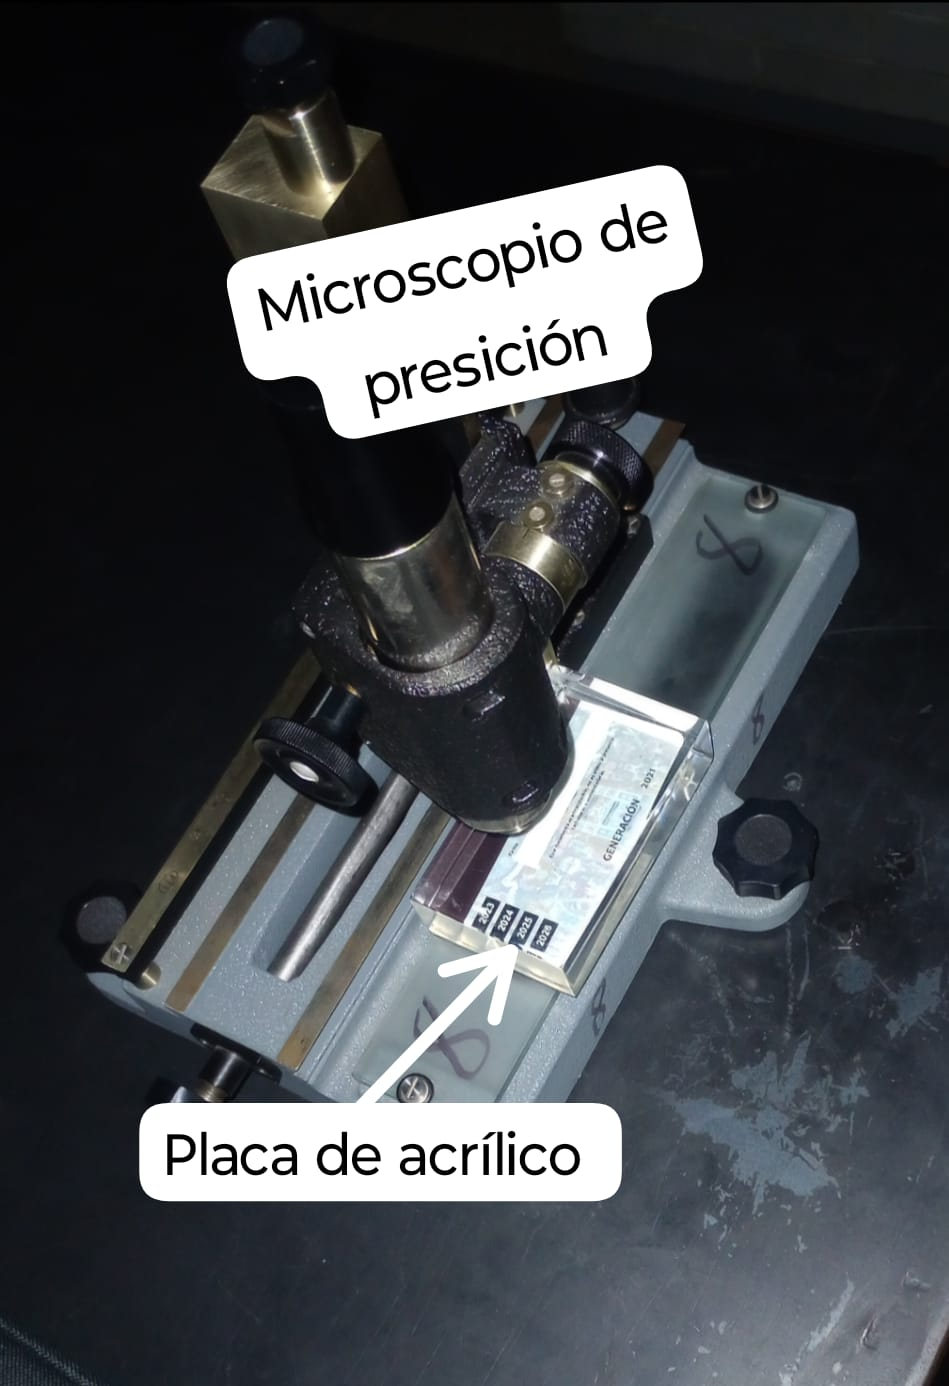
\includegraphics[width=0.2\linewidth]{PPP.png}
    \caption{Arreglo experimental cuando la placa esta sobre la credencial}
    \label{fig:enter-label}
\end{figure}


\subsection*{Método del Prisma}

Colocamos el apice del prisma en el centro del goniométro pero un poco desplazado tal y como se muestra en la figura 5, esto permite que el Lasér entre completamente al prisma manteniendose centrado dentro del eje lo cual nos permite realizar el angulo de desviación de manera más precisa.

\begin{figure}[H]
    \centering
    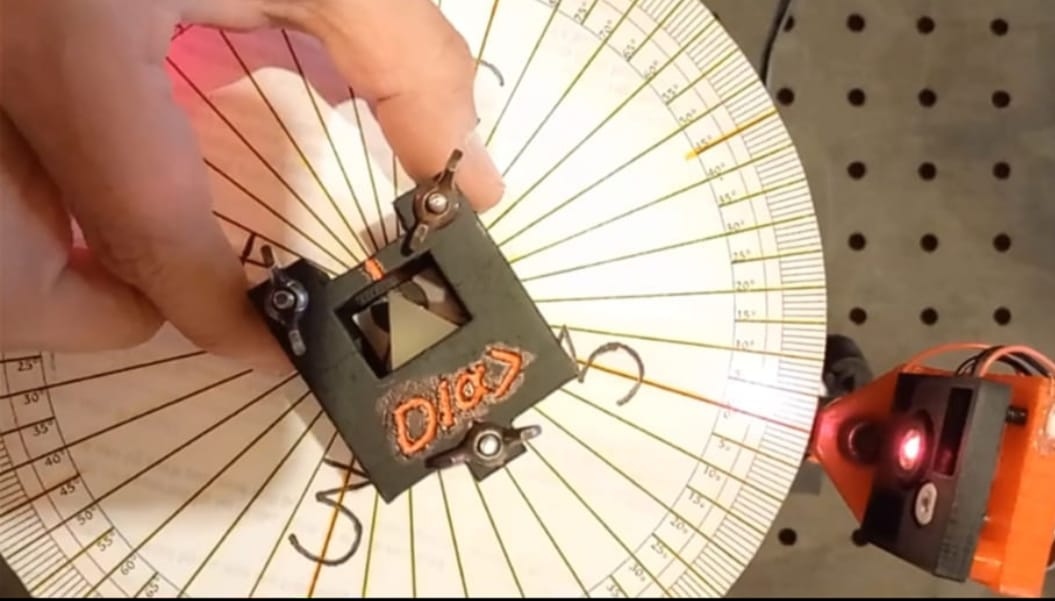
\includegraphics[width=0.5\linewidth]{apice.png}
    \caption{Posición del prisma respecto al centro de goniométro}
    \label{fig:enter-label}
\end{figure}

Luego con ayuda de una pantalla indentificamos el haz desviado por el prisma posteriormente giramos el goniométro mientras seguimos el haz de salida y observamos que este se mueve en una cierta dirección conforme giramos el goniométro hasta que se llega a un cierto punto en el cual este se detiene un momento y e invierte su dirección de movimiento, justo en donde el haz se detiene es en donde se encuentra el angulo de desviación mínima una vez indentificado esté punto, con ayuda de una hoja medimos el ángulo de salida por ultimo cuidando de no mover el goniométro retiramos el prisma y medimos la posición angular en la que sale el haz del goniométro. Con estos dos angulos obtuvimos el angulo de desviación mínima ($\delta_m$) el cual esta dado por la diferencia entre los dos angulos de salida.

\begin{figure}[H]
    \centering
    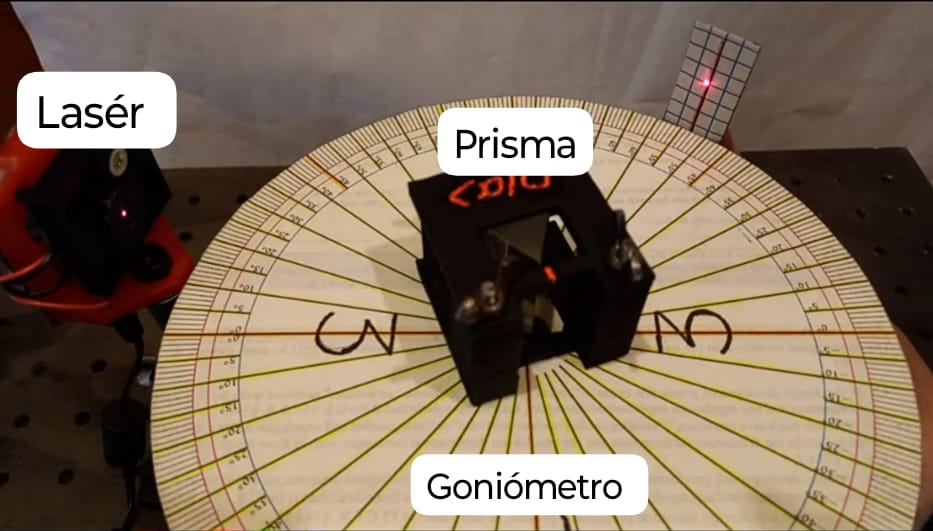
\includegraphics[width=0.5\linewidth]{prima.png}
    \caption{Montaje experimental en el cal se observa el haz desviado debido al prisma}
    \label{fig:enter-label}
\end{figure}

\section{Resultados y tratamiento de datos}
\subsection*{Método de Reflexión Total Interna}


 Se encontró experimentalmente un angulo crítico $\theta_C=43^{\circ}\pm 0.5^{\circ}$ con este dato podemos calcular el índice de refrácción del medio(acrílico) utilizando la ecuación 3 de ángulo crítico \eqref{RTI} del marco teórico, por otro lado calculamos la incertidumbre de n con la ecuacion 9 \eqref{incertidumbre RTI} que encontramos en el apartado del Anexo.


Se midió un ángulo crítico de $\theta_c = 43.0^\circ \pm 0.5^\circ$, a partir del cual se calculó el índice de refracción absoluto del acrílico mediante la ecuación:


\begin{equation}
n_{\text{acrílico}} = \frac{1}{\sin(43^\circ)} = 1.4665 \pm 0.3925
\end{equation}

El valor obtenido concuerda con el índice de refracción esperado para el acrílico ($n \approx 1.49$), aunque la incertidumbre es considerablemente alta (26.7\%). Esto puede deberse a la sensibilidad del método al error en la medición del ángulo crítico, ya que la derivada de la función $\sin^{-1}(\cdot)$ es relativamente grande en este rango angular.\\

La siguiebtes tablas se pueden encontrar en el siguiente enlace \cite{Excel}


\subsection*{Método de Pfund}
\begin{table}[H]
    \centering
    \rowcolors{2}{cyan!20}{yellow!10}
    \begin{tabular}{|c|c|c|c|c|c|}
        \hline
        $D$ (cm) & $\Delta D$ (cm) & $h$ (cm) & $\Delta h$ (cm) & $n$ & $\Delta n$ \\
        \hline
        3.11 & 0.0005 & 0.8500 & 0.001 & 1.48162 & 0.029 \\
        \hline
    \end{tabular}
    \caption{Datos del Método de Pfund}
    \label{tab:pfund}
\end{table}

Podemos observar que en este método obtenemos un índice de refracción n=1.482$\pm$0.029, el índice lo podemos obtener a partir de la ecuación  4 \eqref{Pfound} y la incertidumbre la obtenemos de la ecuación 10 \eqref{incertidumbre Pfound}, el resultado es muy cercano al valor teórico el cual ronda $n= 1.49$


\subsection*{Placa Plano Paralela}
\begin{table}[h]
    \centering
    \rowcolors{2}{cyan!20}{yellow!10}
    \begin{tabular}{|c|c|c|c|c|c|c|c|c|c|c|}
        \hline
        $\theta_i$ (°) & $\Delta\theta_i$ (°) & $X$ (mm) & $D$ (mm) & $\Delta X$ (mm) & $\theta_i$ (rad) & $\sin\theta_i$ & $\cos\theta_i$ & $n$ & $n$ promedio & $\Delta n$ \\
        \hline
        5 & 0.5 & 1.25 & 56.0 & 0.1 & 0.087 & 0.087 & 0.996 & 
 1.342 & & \\
        10 & 0.5 & 2.10 & 56.0 & 0.1 & 0.087 & 0.174 & 0.985 & 1.268 & & \\
        15 & 0.5 & 4.50 & 56.0 & 0.1 & 0.175 & 0.259 & 0.966 & 1.425 & & \\
        20 & 0.5 & 4.80 & 56.0 & 0.1 & 0.262 & 0.342 & 0.940 & 1.300 &1.35 & 0.018\\
        25 & 0.5 & 6.70 & 56.0 & 0.1 & 0.349 & 0.423 & 0.906 & 1.333 & & \\
        30 & 0.5 & 9.25 & 56.0 & 0.1 & 0.436 & 0.500 & 0.866 & 1.387 & & \\
        35 & 0.5 & 10.54 & 56.0 & 0.1 & 0.524 & 0.574 & 0.819 & 1.347 & & \\
        40 & 0.5 & 13.80 & 56.0 & 0.1 & 0.611 & 0.643 & 0.766 & 1.399 & & \\
        \hline
    \end{tabular}
    \caption{Datos del Método de Placa Plano Paralela}
    \label{tab:placa}
\end{table}
Podemos observar que por el método de placas plano paralelas se obtuvo un índice de refracción $n=1.35\pm0.018$ el cual se obtuvo a partir de la ecuación 6 \eqref{PPP} y su incertidumbre de la ecuación 12 \eqref{incertidumbre PPP}, el valor del índice es similar al teórico ($n_{H_2O}=1.333$)

\subsection*{Profundidad Aparente}
\begin{table}[H]
    \centering
    \rowcolors{2}{cyan!20}{yellow!10}
    \begin{tabular}{|c|c|c|c|c|c|c|c|}
        \hline
        Sobre (cm) & Bajo (cm) & Sin (cm) & $\Delta$ (cm) & $r$ (cm) & $a$ (cm) & $n$& $\Delta n$ \\
        \hline
        6.11 & 4.55 & 3.79 & 0.0005 & 2.32 & 1.56 & 1.487& 0.001\\

        \hline
    \end{tabular}
    \caption{Datos del Método de Profundidad Aparente}
    \label{tab:profundidad}
\end{table}

Por el método de profundidad aparente el índice de refracción resultante es $n=1.487\pm0.001$ el cual se obtiene de la ecuación 5 \eqref{P.A} y su incertidumbre de la ecuación 11 \eqref{incertidumbre P.A} que se encuentra del anexo, podemos observar que el valor obtenido es cercano al teórico $n = 1.52$

\subsection*{Método del Prisma}
\begin{table}[H]
    \centering
    \rowcolors{2}{cyan!20}{yellow!10}
    \begin{tabular}{|c|c|c|c|c|}
        \hline
        $\delta_m$ (°) & $\Delta\delta_m$ (°) & $\alpha$ (°) & $n$&$\Delta n$ \\
        \hline
        66.0 & 0.5 & 60° & 1.782&0.045 \\
        \hline
    \end{tabular}
    \caption{Datos del Método del Prisma}
    \label{tab:prisma}
\end{table}

Por último por el método del prisma el índice de refraccíon es $n=1.782\pm0.045$ el cual se obtiene de la ecuación 7 \eqref{Prisma}y su incertidumbre de la ecuación 13 \eqref{incertidumbre prisma}, el cual es muy cercano al teórico (n=1.776).



\section{Conclusiones}

\begin{enumerate}
    \item \textbf{Precisión y confiabilidad de los métodos}  
    El método de \textbf{Profundidad Aparente} resultó ser el más preciso, con un índice de refracción de $n = 1.487 \pm 0.001$, muy cercano al valor teórico y con la menor incertidumbre. En contraste, el método de \textbf{Reflexión Total Interna} presentó la mayor incertidumbre (26.7\%), lo que indica que pequeñas variaciones en el ángulo crítico afectan considerablemente el resultado.
    
    \item \textbf{Exactitud de los valores obtenidos}  
    Todos los métodos dieron valores de $n$ cercanos a los valores teóricos esperados, con diferencias dentro del margen de error experimental. El método del \textbf{Prisma} arrojó un resultado muy preciso ($n = 1.782 \pm 0.045$), lo que confirma su efectividad para medir índices de refracción con alta exactitud.
    
    \item \textbf{Fuentes de error}  
    Los principales errores provinieron de la medición de ángulos y desplazamientos, así como la alineación del láser y la calidad del material utilizado. En el método de \textbf{Placa Plano Paralela}, el resultado fue menor al teórico ($n = 1.31 \pm 0.014$ en comparación con $n = 1.333$), lo que sugiere posibles errores sistemáticos en la medición del desplazamiento lateral del haz.
    
    \item \textbf{Importancia del estudio del índice de refracción}  
    La medición del índice de refracción es fundamental en óptica y tiene aplicaciones en lentes, espejismos y otros fenómenos ópticos. Los resultados obtenidos permiten validar la Ley de Snell y la teoría de la refracción en distintos materiales.
\end{enumerate}

En general, los valores obtenidos en la práctica fueron satisfactorios y permiten concluir que los métodos experimentales utilizados son efectivos para la medición del índice de refracción, aunque algunos requieren mayor precisión en la medición de ángulos y alineación del equipo.

 



\begin{thebibliography}{9}
    \bibitem{snell} E. Hecht, \textit{Óptica}, Addison Wesley, 3ª Edición, 2000.
    \bibitem{indice_ref} Erick Barrios Barocio, Roxette Ramírez Arvidez, \textit{Medición del Índice de Refracción}, Óptica v.2025.
       \bibitem[]{Excel} A. Reyes, S. Tablas de Índice de Refracción, Archivo Excel. 2024. Disponible en: \href{https://docs.google.com/spreadsheets/d/1aX8uVuEyiOjETpa2oIGZVDQLiuMoqKv-/edit?usp=sharing&ouid=112625838925660900694&rtpof=true&sd=true}{Enlace al documento}
\end{thebibliography}



\subsection*{Anexo}

Incertidumbre nominal para la ecuación del ángulo crítico (Reflexión total interna) \eqref{RTI}

\begin{mdframed}
    \label{incertidumbre RTI}
\begin{equation}
    \Delta n = \left| \frac{dn}{d\theta_c} \right| \cdot \Delta \theta_c = \left| -\frac{\cos(\theta_c)}{\sin^2(\theta_c)} \right| \cdot \Delta \theta_c
\end{equation}
\end{mdframed}

Incertidumbre nominal para la ecuación del método de Pfound \eqref{Pfound}

\begin{mdframed}
 \label{incertidumbre Pfound}
    \begin{equation}
        \sigma_{np}=\sqrt{(\frac{16h^{2}\Delta D}{D{^2}\sqrt{D^{2}+16h^{2}}})^{2}+(\frac{16h \Delta h}{\sqrt{D^{2}+16h^{2}}})^{2}}
    \end{equation}
\end{mdframed}

Incertidumbre nominal para la ecuación de profundidad aparente \eqref{P.A}
\begin{mdframed}
    \label{incertidumbre P.A}
    \begin{equation}
        \sigma_{ni}= \sqrt{(\frac{\Delta r}{a})^{2}+(\frac{r\Delta a}{a^{2}})^2}
    \end{equation}
\end{mdframed}

Incertidumbre  para la ecuación de Placas de Plano Paralelas \eqref{PPP}

\begin{mdframed}
 \label{incertidumbre PPP}
 \begin{equation}
\sigma_{est}=\sqrt{\frac{\sum_{i=1}^{N}(n_i-\bar{n})^2}{N(N-1)}}
\end{equation}
   
\end{mdframed}

Incertidumbre para la ecuación del método del prisma \eqref{Prisma}

\begin{mdframed}
    \label{incertidumbre prisma}
    \begin{equation}
        \sigma_n= \frac{cos(\frac{\delta_m+\alpha}{2})}{2sen(\frac{\alpha}{2})}
    \end{equation}
\end{mdframed}







\end{document}